\documentclass[14pt,fleqn]{extarticle}
\RequirePackage{prepwell}

\previewoff 

\begin{document} 
\begin{skill}
    \begin{narrow}
         \textcolor{blue}{Injective, Surjective \& Bijective} 
         
         Types of functions. Easy concepts, difficult names
    \end{narrow}
    
    \reason 
    
    The figure below shows the various types of functions you need 
    to know about 
    
    \begin{center}
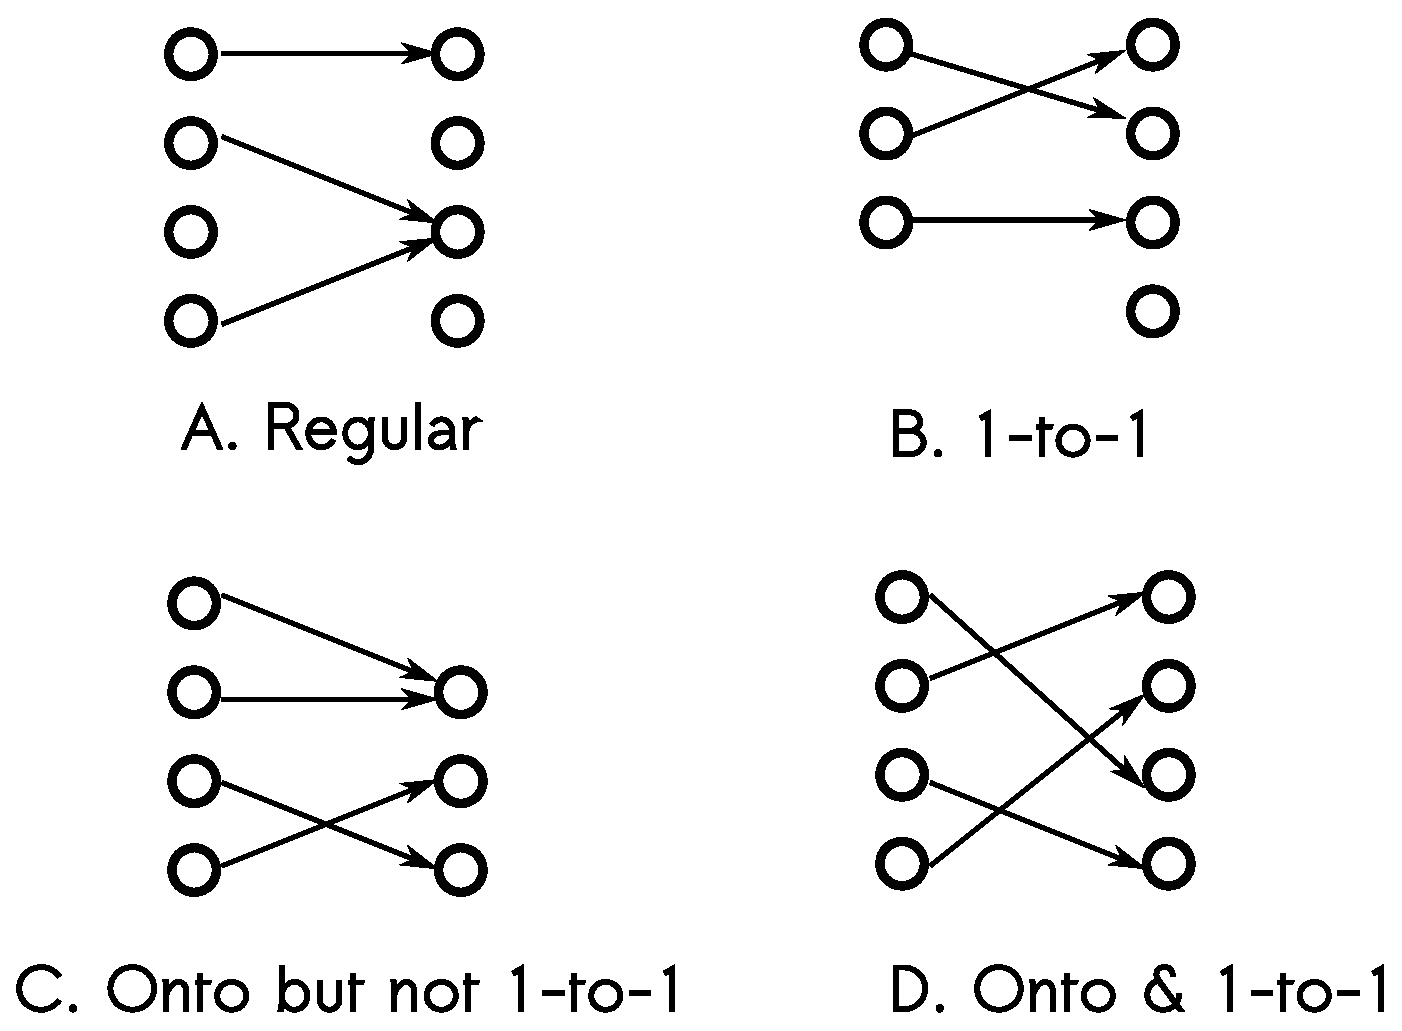
\includegraphics[scale=0.33]{142-A.eps}
\end{center}
    
    \begin{center}
  \begin{tabular}{Nlll}
   \toprule
        & Name & Type & Bear in mind \\
   \midrule 
   A & & Regular & Two $x$ can map to\\
   & & & the same $y$ but one $x$\\
   & & & cannot map to two $y$ \\
    \midrule
  B & Injective & 1-to-1 & $f(x) = f(y) \implies x = y$ \\
  & & & $f(x)\neq f(y)\implies x \neq y$ \\
  \midrule 
  C & Surjective & Onto & Every $y$ in co-domain is\\
  & & & mapped to some $x$ in domain  \\
  \midrule 
  D & Bijective & Invertible & Injective $+$ Surjective\\  
    \bottomrule
  \end{tabular}
\end{center}
\end{skill}
\end{document} 